% Chapter 5

\chapter{Implementation} % Main chapter title
\label{Chapter5} % For referencing the chapter elsewhere, use \ref{Chapter1} 

\lhead{Chapter 5. \emph{Implementation}} % This is for the header on each page - perhaps a shortened title

This chapter explores the implementation aspects of the regression algorithms discussed in Chapter \ref{Chapter4}. The implementation goal is to have \textit{learners} (running learning algorithm instances), based on the previously covered regression algorithms, that fulfill the requirements listed in \ref{list:restimator_requirements}. Most of the effort put in the implementation of the learners is to meet the second requirement which is \textit{robustness to abrupt concept drifts}. As discussed in \ref{subsection:2.4.1}, learners with the ability to adapt to non-stationary streaming data are called online learners. From the implementation point of view, the most essential feature of an online learner is the \textit{incremental update mechanism} that affords the required adaptivity to the non-stationarity. Therefore, the main focus of this Chapter is on the implementation of the incremental update mechanism for the the regression algorithms discussed previously. 

Since none of the regression algorithms covered in the previous chapter is originally proposed with an in-built incremental update mechanism, their prediction mechanism should be \textit{reimagined} so that they can incrementally update their internal predictive models with the new data points arriving from the data stream. Undoubtedly, the incremental update mechanism for different learning algorithm should be implemented using different techniques due to the different prediction mechanisms they feature. Hence, before discussing the implementation of update mechanism employed in the implemented online learners, a categorization of the regression algorithms based on the way they build their predictive model and come up with prediction bounds is presented. 

\section{Categorization of Regression Algorithms}

In how regression algorithms treat the input to build a predictive model, they are divided into two classes namely \textit{absorbing methods} and \textit{accumulative methods}. The parametric algorithms discussed in Chapter \ref{Chapter4}, MAP-method and MLE-method, are absorbing methods. They infer the parameters of the regression function from the observed data and make predictions with the parameters inferred. More precisely, the observed data play no direct role in making predictions. On the other hand. non-parametric algorithms covered, Gaussian Process Regression and Kernel Regression, are data-driven methods. They accumulate the data to deliver predictions. More precisely, In non-parametric regression algorithms, the predicted target for a new point can be formulated as the weighted average of the observed targets for the accumulated data points that.

For the main regression algorithms considered in this thesis, the absorbing methods and the accumulative methods nicely correspond to parametric learning models and non-parametric ones respectively. However, this holds only when the algorithms are used to make point predictions. If prediction bounds along with the point predictions are needed, the prediction bounds estimation mechanism should also be considered before deciding an algorithm needs to store the historic data or not. 

From the non-parametric learning models, Gaussian Process Regression finds the predictive variance by using only the design matrix which is composed of only the inputs of the past data (\ref{def_4.25}). On the other hand, Kernel Regression needs to calculate the \textit{instantaneous} squared residual error\footnote{Instantaneous squared residual error is the measure of amount of error that the updated version of the online learner \textit{would} make for the past data points.} for the historic data points prior to the estimation for new data point (\ref{def_4.42}) necessitating the bookkeeping of the past observed targets. However, for making the point predictions, since both of these algorithms already need to store both the inputs and the observed targets of the historic data (\ref{def_4.25}, \ref{def_4.41}), their prediction bound estimation mechanism do not impose any additional data storage requirements. 

For the parametric models, as their prediction mechanism itself does not require storing any of the past data, the choice for the prediction bound estimation mechanism determines the data storage requirements. Finding the asymptotic prediction intervals for MLE-method discussed in \ref{subsubsection:4.2.1.2} requires the computation of the instantaneous squared residual error just like the prediction bounds estimation method of Kernel Regression. Since computing the instantaneous squared residual error computation requires the observed targets of the past data points, the absorbing methods which use this prediction bound estimation method have to store them. As an alternative to the asymptotic prediction bounds, an ad-hoc prediction bounds estimation method\footnote{This is a fully practical method without any theoretical support and it is referred to as ad-hoc prediction bounds estimation method. Its details is discussed in \ref{subsubsection:impl_predict_mleforgetting}} that is not based on the instantaneous squared residual error is implemented to be employed for parametric algorithms. Due to these two options for the prediction bound estimation method, two different sets of online learners based on parametric models are implemented. One set implements the ad-hoc prediction bounds method that do not require storing any of the historical data and the other set implements the asymptotic prediction bounds estimation method.

\section{Categorization of Online Learners}

Having discussed the dependencies of the online learning algorithms on the data when making point predictions and estimating prediction bounds, it is possible to propose two different types of design for the online learners to be implemented to handle stream data with potential non-stationaries. These are the forgetting-based design and sliding-windowed design.

\subsection{Forgetting-based Design}

Forgetting-based design is for the learning algorithms that do not need to store the past data for their point prediction and prediction bounds estimation mechanism. This kind of design is applicable to online learners based on parametric regression algorithms. The main idea is to discount the effect of the less recent data points on the calculation of the parameters by means of a forgetting-factor parameter, denoted as $\alpha$. In order to make this possible a recursive parameter computation method parameterized with $\alpha$ is needed. Borrowing some of the ideas presented in \citep[pp. 161-164]{bontempi_statistical_2011}, the needed formula is derived as follows.
\begin{align*}
\text{let } \pmb{w}_{old} & = (XX^{\top})^{-1}X\pmb{y} = M1_{old}M2_{old} \numberthis \label{def_5.1} \\
\pmb{w}_{new} & = ([X \ \pmb{x}_{new}][X \ \pmb{x}_{new}]^{\top})^{-1}[X \ \pmb{x}_{new}] [\pmb{y} \ y_{new}]^{\top} \\
M1_{new}^{-1} & = [X \ \pmb{x}_{new}][X \ \pmb{x}_{new}] = XX^{\top} + \pmb{x}_{new}\pmb{x}_{new}^{\top} \\ 
& = M1_{old}^{-1} + \pmb{x}_{new}\pmb{x}_{new}^{\top} \text{ (rank-1 update) } \numberthis \label{def_5.2} \\
M2_{new} & = [X \ \pmb{x}_{new}][\pmb{y} \ y_{new}]^{\top} = M2_{old} + \pmb{x}_{new}y_{new} \\
M1_{old}^{-1}\pmb{w}_{old} & = (XX^{\top})^{-1}(XX^{\top})^{-1}X\pmb{y} = X\pmb{y} \\
M1_{new}^{-1}\pmb{w}_{new} & =  [X \ \pmb{x}_{new}][\pmb{y} \ y_{new}] = M1_{old}^{-1}\pmb{w}_{old} + \pmb{x}_{new}y_{new} \\
& = (M1_{new}^{-1} - \pmb{x}_{new}\pmb{x}_{new}^{\top})\pmb{w}_{old} + \pmb{x}_{new}y_{new} \text{ (using } \ref{def_5.2}) \\
& = (M1_{new}^{-1}\pmb{w}_{old} - \pmb{x}_{new}\pmb{x}_{new}^{\top}\pmb{w}_{old} + \pmb{x}_{new}y_{new} \\
& = (M1_{new}^{-1}\pmb{w}_{old} - \pmb{x}_{new}(y_{new} - \pmb{x}_{new}^{\top}\pmb{w}_{old}) \\
\pmb{w}_{new} & = \pmb{w}_{old} - M1_{new}\pmb{x}_{new}(y_{new} - \pmb{x}_{new}^{\top}\pmb{w}_{old}) \text{ where; }   \numberthis \label{def_5.3} \\
M1_{new} & = (M1_{old}^{-1} + \pmb{x}_{new}\pmb{x}_{new}^{\top})^{-1} \text{ (using } \ref{def_5.2}) \\
M1_{new} & = M1_{old} - \frac{M1_{old}\pmb{x}_{new}\pmb{x}_{new}^{\top}M1_{old}}{1+\pmb{x}_{new}^{\top}M1_{old}\pmb{x}_{new}} \text{ (using matrix inversion lemma \cite{bartlett_inverse_1951})} \numberthis \label{def_5.4} \\
& \text{Plugging \ref{def_5.4} into \ref{def_5.3}; } \\
\pmb{w}_{new} & = \pmb{w}_{old} - (XX^{\top})^{-1} - \frac{(XX^{\top})^{-1}\pmb{x}_{new}\pmb{x}_{new}^{\top}(XX^{\top})^{-1}}{1+\pmb{x}_{new}^{\top}(XX^{\top})^{-1}\pmb{x}_{new}})\pmb{x}_{new}(y_{new} - \pmb{x}_{new}^{\top}\pmb{w}_{old}) \numberthis \label{def_5.5}
\end{align*}
The equation \ref{def_5.5} is recursive, therefore a new data point (denoted as $\pmb{x}_{new}$ can be easily used to update the parameters from $\pmb{w}_{old}$ to $\pmb{w}_{new}$. However, the forgetting factor, $\alpha$, is not used in \ref{def_5.5} to discount the effect of less recent data points on the parameters. The following modification of the formula that calculates the first multiplicand, $M1$, of the parameter vector to be estimated is done to introduce the forgetting factor into the calculation.
\begin{align*}
M1_{new} & = \frac{1}{1-\alpha}(M1_{old} - \frac{M1_{old}\pmb{x}_{new}\pmb{x}_{new}^{\top}M1_{old}}{1+\pmb{x}_{new}^{\top}M1_{old}\pmb{x}_{new}}) \numberthis \label{def_5.6}
\end{align*}
Plugging \ref{def_5.6} into \ref{def_5.3} and writing only in terms of data points and their corresponding observed targets, the following parameter estimation formula parametrized with a forgetting factor $\alpha$ is obtained.
\begin{flalign}
\pmb{w}_{new} & = \pmb{w}_{old} - \frac{1}{1-\alpha}((XX^{\top})^{-1} - \frac{(XX^{\top})^{-1}\pmb{x}_{new}\pmb{x}_{new}^{\top}(XX^{\top})^{-1}}{1+\pmb{x}_{new}^{\top}(XX^{\top})^{-1}\pmb{x}_{new}})\pmb{x}_{new}(y_{new} - \pmb{x}_{new}^{\top}\pmb{w}_{old})) \label{def_5.7}
\end{flalign}

Forgetting-based design ensures the adaptivity to the emerging concepts by discounting the effect of the $m_{th}$ most recent data point by $\alpha^{m-1}$ favoring the newer data points over the older ones.

Online learners using forgetting-based design cannot tune themselves as all the tuning schemes require access to data.

\subsection{Sliding-Window Design}

Sliding-window design can be used for learning algorithms that depend on the past data for either making point predictions or estimating the prediction bounds. The main idea is to store most recent $k$ data points in most-recent to least-recent order in a structure called sliding window. Moreover, with every new data point arrive from the stream, the least recent data point from the tail of the window is dropped and the window items are slid by one position to the tail making space for the most recent data point in the head position of the stream. The data available to the learning algorithm for delivering predictions with prediction bounds is the data stored in the sliding-window. As sliding window stores the most recent data points, the adaptation to emerging concepts is automatic. Furthermore, as the sliding-window size is fixed throughout the lifetime of the online learner, the space it occupies can always be bounded by a constant which is a desirable property in online learning scenario.

The operation of the sliding-window on a data stream is illustrated in \ref{fig:streaming}

\begin{figure}[htbp]
  \centering
    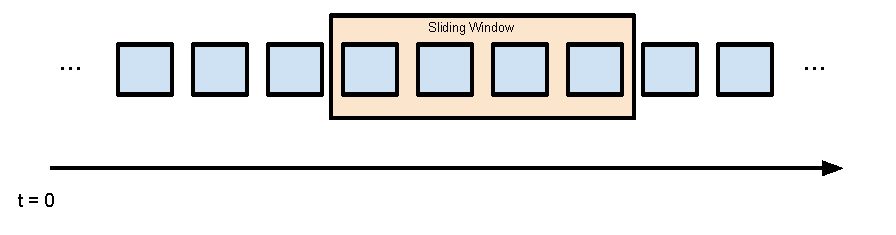
\includegraphics[width=\linewidth]{./Figures/streaming.pdf}
  \caption{Sliding window on a data stream is visualized}
  \label{fig:streaming}
\end{figure}

In order to realize the mentioned \textit{sliding} operation (costly if implemented in a naive way) with the new data points arriving, a ring buffer is employed making it possible to \textit{slide} the window by only modifying two pointers that point to beginning end the end of the buffer.

\section{Online Learner Semantics}
\label{section:online_learner_semantics}

There are two basic functionality that all the online learners should implement. These are \texttt{predict}, and \texttt{update}. Moreover, there is one more optional operation that is implemented only by the sliding-windowed online learners. This operations is called \texttt{tune} and it \textit{calibrates} the online learner by using the data stored in the sliding window. The behavior of the online learners are determined by their current state. The frequency they carry out these two mandatory and one optional operations change from one state to another. In order to capture these different behaviors, state transitions for forgetting-based learners and the sliding-windowed learners are presented.

\begin{figure}[htbp]
  \centering
    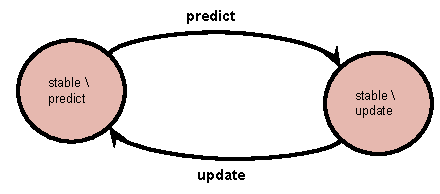
\includegraphics[width=\linewidth]{./Figures/forgetting-based_states.pdf}
  \caption{State-transition diagram of the forgetting-based learners}
  \label{fig:forgetting-based_states}
\end{figure}

Figure \ref{fig:forgetting-based_states} describes the states, state transition invoking operations and the order by which different kind of operations follow each other for the forgetting-based learner implementations. According to the diagram, there are simply two states where the learner is allowed to carry out one of the \texttt{update} or \texttt{predict} operations. These two operations always follow each other. It is easy to \textit{play} the online prediction protocol whose pseudocode is presented in pseudocode \ref{alg:opp} on this state diagram.

\begin{figure}[htbp]
  \centering
    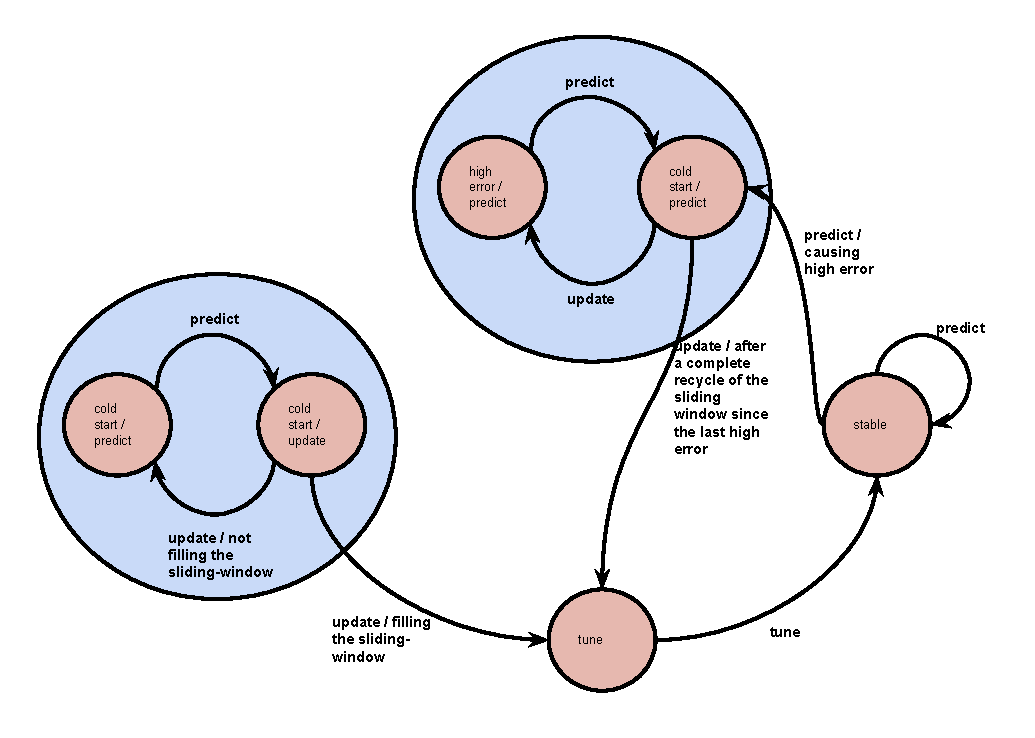
\includegraphics[width=\linewidth]{./Figures/sliding-windowed_states.pdf}
  \caption{State-transition diagram of the sliding-windowed learners}
  \label{fig:sliding-windowed_states}
\end{figure}

Figure \ref{fig:forgetting-based_states} describes the states, state transition invoking operations and the order by which different kind of operations follow each other for the sliding-windowed learner implementations. Their state-transition diagram is more complex than that of forgetting-based learners. According to the diagram, a sliding-windowed learner is in one of the four main state namely cold start, stable, high-error and tune. There are two mini-states within the cold start and high-error states where the predictions and updates successively follow each other conforming to online prediction protocol (pseudocode \ref{alg:opp}). However, in the state stable after transiting from the one-operation state tune, the learner is not updated with the new data as long as its predictions are accurate. The reason for such a design choice is that for the sliding-windowed learners the \texttt{update} is a costly operation involving matrix manipulations. Therefore, whenever it is not necessary, it can be skipped to speed up the online learner. When the prediction error for predicted data points is low, this means that the learner has adapted to the current concept and its current model will perform well until a new concept is encountered in the data stream. When a concept drift occurs, this is detected by the increasing prediction error and the learner transits to high-error state where each \texttt{predict} operation is followed by an \texttt{update} operation. And this high-error state lasts until all the data points left from the pre-high-error detection is replaced by the newer ones. Then, tuning takes place where the hyperparameters of the learning algorithms are fine-tuned. The cold-start state is very similar to high-error state however, differently, in the cold-start state, the sliding window implemented by a ring buffer only incorporates the data points arriving from the stream and do not drop any until the sliding window gets full. Then the learner tunes itself and winds up in the stable state.

\section{Implementation of Online Learner Operations}

In this section, the implementation of the \texttt{predict}, \texttt{update} and \texttt{tune} operations for each online regression algorithm discussed in Chapter \ref{Chapter3} are presented. Moreover, the computational shortcuts proposed in the literature for recursive fast-update routines are discussed for the applicable regression algorithms. Furthermore, the prediction bounds estimation methods that are not covered in Chapter \ref{Chapter4} due to the their lack of theoretical support is discussed here.

\subsection{MLE method operations}

MLE method, being a parametric algorithm, could be implemented using either forgetting-factor design or sliding-windowed design. Obviously, the implementation of the \textit{predict}, \textit{update} and \textit{tune} operations depend on this design choice. Next, the implementation of each operator for both of the design choices is discussed.

\subsubsection{Implementation of \texttt{predict} for \texttt{BayesianMLEForgetting}}
\label{subsubsection:impl_predict_mleforgetting}

Point predictions mechanism of \texttt{BayesianMLEForgetting} is simple once the regression parameters vector $\pmb{w}$ is known. The point prediction is simply the product of parameters, $pmb{w}$ and the data point, $\pmb{x}$, for which the target is predicted.

In the case feature-space mapping is opted in, the input is mapped to the feature space by the set of base functions defined. The set of base functions implemented is formulated as follows.
\begin{align*}
 \Phi(\pmb{x}) = \{\phi: y = \phi(\pmb{x}) = \pmb{x}_i^a\pmb{x}_j^b \ | \ \forall y \in \mathcal{R} \wedge \forall \pmb{x} \in \mathcal{R}^d \wedge \forall i,j \in \mathcal{R}_{> 0} \\ \wedge \ \exists a,b \in \mathcal{R}_{\geq 0} \wedge i \leq d \wedge j \leq d \wedge 1 \leq a+b \leq 2\}
 \end{align*}
Above, i and j are the indices of the values that sit at respectively the $i_{th}$ and $j_{th}$ dimension of the input vector \pmb{x}. In addition to the base functions expressed above, logarithm and square root of each dimension of the input vector is used as additional base functions. Feature-space mapping is oblivious to learning algorithm used. It is used by the half of the parametric learners. When it is used the number of parameters increase from $d$ to the cardinality of above described set plus $2d$ (because of the addition of the logarithm and square root base functions). In the rest of this chapter, the feature-space mapping implementation is not separately discussed for different learners other than \texttt{BayesianMLEForgetting} as they all share the same implementation.

As for estimating the prediction bounds for the data point which a point prediction is made for, the asymptotic prediction intervals by the MLE-method is not applicable as that method requires access to the past observed targets and forgetting-based method do not store any historic data. This is why, the previously mentioned ad-hoc prediction bounds idea is proposed to make prediction bound estimations without needing the historic data. The idea is maintaining three versions of the online learner one of which is called \textit{base} learner and the other two are upper bound learner and lower bound learner. The learner system consists of these three learners is called \textit{3-learner ensemble}. The point predictions made by the base learner is returned as the point prediction for a data point for which the target prediction is requested. As for bound learners, the point prediction of the upper bound learner constitutes the upper bound of the prediction. Likewise, the point prediction by the lower bound learner constitutes the lower bound of the prediction. In order to make this prediction scenario possible, these three learners should be updated with different set of data points after a predefined \textit{burn-in} time. After that, the upper bound learner is updated with the data points with observed targets that are higher than the the lower bound prediction made made by the 3-learner ensemble. Similarly, the lower bound learner is updated with the data points with observed targets that are lower than the the upper bound prediction made by the 3-learner ensemble. This idea is sketched in \ref{fig:ad-hoc_prediction_bounds}.

\begin{figure}[htbp]
  \centering
    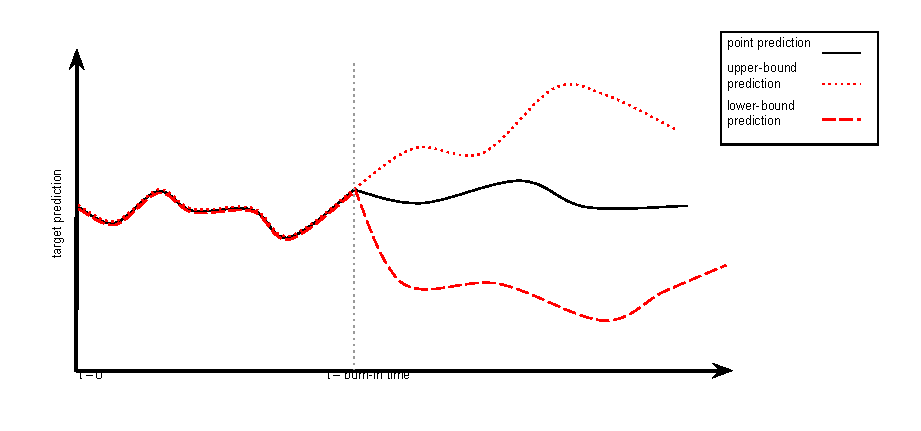
\includegraphics[width=\linewidth]{./Figures/ad-hoc_prediction_bounds.pdf}
  \caption{Ad-Hoc prediction bounds method is illustrated}
  \label{fig:ad-hoc_prediction_bounds}
\end{figure}

\subsubsection{Implementation of \texttt{update} for \texttt{BayesianMLEForgetting}}
\label{subsubsection_impl_update_bmleforgetting}

Implementation of \texttt{update} operation depends on the previously derived recursive version of parameter calculation formula, \ref{def_5.7}. However, the concrete implementation should define an initial matrix for $X_0X_0^{\top}$. \citep[pp. 162-163]{bontempi_statistical_2011} suggests that the initial $X_0X_0^{\top}$ matrix should be in the form of $kI$ where $k$ is some constant. It is also suggested that $k$ should be chosen to be high if the parameters estimated using the recursive formulation is preferred to diverge from the initial conditions quickly. Therefore, the constant $k$ is chosen to be $10000$. It is also worth noting that starting with $kI$ as the initial matrix guarantees that $XX^{\top}$ will be invertible in the following recursive steps.

\subsubsection{Implementation of \texttt{predict} for \texttt{BayesianMLEWindowed}}

Once the parameters $\pmb{w}$ is ready, making a point prediction takes simply multiplying the parameters and the data point whose unobserved target needs to be estimated.

Estimating the prediction bounds using the asymptotic prediction bound estimation method is formulated in \ref{def_4.17}. As previously discussed, \ref{def_4.17} includes the term $s^2$ which is the instantaneous squared residual error. Assuming the instantaneous squared residual error is computed in the previous \textit{update} operation, finding the prediction bounds by evaluating \ref{def_4.17} is straightforward.

\subsubsection{Implementation of \texttt{update} for \texttt{BayesianMLEWindowed}}
\label{subsubsection:update_bmlewindowed}

The operation \texttt{update} for \texttt{BayesianMLEWindowed} involves two different sub-operations. These are updating the parameters and recomputing the instantaneous squared residual error. The first operation is twofold. First, the effect of the oldest data point in the (already full) sliding window should be removed from the parameters. Then, the new data point should be \textit{absorbed} into the parameters. These two sub-operations can be done using rank-1 downdate and rank-1 update of $M_1^{-1}$ matrix respectively. Additionally $M2$ should be downdated and updated accordingly. The derived parameter update formula in \ref{def_5.5} only addresses the \textit{update} part of the operation and it lacks the downdate part. Therefore, the following parameter downdate equation is derived.
\begin{align*}
\pmb{w}_{old} & = (XX^{\top})^{-1}X\pmb{y} = M1_{old}M2_{old} \\
M1_{old}^{-1} & = [\pmb{x}_k \ \pmb{x}_{k+1} \ ... \ \pmb{x}_{k+w-1}][\pmb{x}_k \ \pmb{x}_{k+1} \ ... \ \pmb{x}_{k+w-1}]^{\top} \\
M1_{new}^{-1} & = [\pmb{x}_{k+1} \ ... \ \pmb{x}_{k+w-1}][\pmb{x}_{k+1} \ ... \ \pmb{x}_{k+w-1}]^{\top} \\
& = M1_{old}^{-1} - \pmb{x}_{k}\pmb{x}_{k}^{\top} \text{ rank-1 downdate, analogous to \ref{def_5.2} } \numberthis \label{def_5.8} \\
M1_{new} &= M1_{old} + \frac{M1_{old} \pmb{x}_{k}\pmb{x}_{k}^{\top} M1_{old}}{1 - \pmb{x}_{k}^{\top} M1_{old} \pmb{x}_{k}} \text{ (using matrix inversion lemma \cite{bartlett_inverse_1951} on \ref{def_5.8})} \numberthis \\
M2_{old} & = [\pmb{x}_k \ \pmb{x}_{k+1} \ ... \ \pmb{x}_{k+w-1}][y_k \ y_{k+1} \ ... \ y_{k+w-1}]^{\top} \\
M2_{new} & = [\pmb{x}_{k+1} \ ... \ \pmb{x}_{k+w-1}][y_{k+1} \ ... \ y_{k+w-1}]^{\top} \\
& = M2_{old} - \pmb{x}_k y_k \numberthis \label{def_5.10} \\
\pmb{w}_{new} & = M1_{new}M2_{new} \numberthis \label{def_5.11}
\end{align*}
Above, w denotes the size of the sliding window. For downdating \ref{def_5.11} can be used. Thus, the downdating requires to recursively update two stored matrices namely $M1$ and $M2$. The initialization of $M1$ is done as explained in \ref{subsubsection_impl_update_bmleforgetting}. On the other hand, $M2$ can be initialized as a zero column matrix. It is worth noting that the derived downdate formula can be adapted to rank-1 update scenario for updating as an alternative to the \ref{def_5.5} formula for updating. Two formulas are essentially the same.

Only variable the time spent by update and downdate sub-operations for the matrix operations involved in \ref{def_5.10}} and \ref{def_5.2} depends on is $n$ which is the input space dimensionality. Since the for a given learning problem, $n$ is fixed, the time spent by these operations can be bounded by a constant.

As for the second operation mentioned, recalculation of the instantaneous squared residual error is straightforward. After obtaining the new parameters following the downdate and update mentioned, for each data point stored, a new point prediction is made and the squared difference of each of the predictions from the corresponding observed stored response is summed up. This requires one pass over the stored data points and their corresponding responses. The length of this pass is simply the size of the sliding window which is $w$. Since the sliding window-size is a constant, the time required for the described one-pass routine can be bounded by a constant.

\subsubsection{Implementation of \texttt{tune} for \texttt{BayesianMLEWindowed}}

\texttt{BayesianMLEWindowed} does not depend on a hyperparameter to be tuned. Although the learner inherits all the features of sliding-windowed learners and also follows the state transition diagram of them, its tuning method is an empty method.

\subsection{MAP method operations}

MAP-method implementation is very similar to that of MLE-method. Hence, this section frequently refers to the previous section.

\subsubsection{Implementation of \texttt{predict} for \texttt{BayesianMAPForgetting}}

The \texttt{predict} operation does the same as its \texttt{BayesianMLEForgetting} counterpart for making point predictions. It simply returns the multiplication of the parameter vector that represents the previously calculated parameters and transpose of the matrix that represents the datapoint. Furthermore, for estimating the prediction bounds,  \texttt{BayesianMAPForgetting} uses the ad-hoc prediction bounds estimation method like \texttt{BayesianMLEForgetting} does.

\subsubsection{Implementation of \texttt{update} for \texttt{BayesianMAPForgetting}}

The implementation of the \textit{update} operator of \texttt{BayesianMAPForgetting} is exactly same as that of \texttt{BayesianMLEForgetting}. However, how the matrix $X_0X_0^{\top}$ is initialized is different. Instead of using $kI$ as the initial $X_0X_0^{\top}$ matrix, \texttt{BayesianMAPForgetting} uses $\sigma_y^2 \Sigma_w^{-1}$ as implied by the equation \ref{def_4.19}. This difference, initializing the $XX^{\top}$ with the regularization term does not have any procedural implications. In other words, \texttt{update} operation runs exactly in the same way as it does in \texttt{BayesianMLEForgetting}.

\subsubsection{Implementation of \texttt{predict} for \texttt{BayesianMAPWindowed}}

\texttt{BayesianMAPWindowed} learners make point predictions by calculating the product of parameters and the data point just as any other parametric learner does. As for estimating prediction bounds, the available theoretically sound methods for MAP-method are not practically suitable for the online learning scenario due to their high complexity as discussed in \ref{subsubsection:map_pred_bounds}. As an alternative, the asymptotic prediction bound estimation method for MLE-method is used.

\subsubsection{Implementation of \texttt{update} for \texttt{BayesianMAPWindowed}}

The implementation of \texttt{update} operation for \texttt{BayesianMAPWindowed} is exactly same as the implementation of \texttt{update} operation for \texttt{BayesianMLEWindowed}. Once the initialization of $XX^{\top}$ is done with the regularization term (different than the initialization for \texttt{BayesianMLEWindowed}) as discussed in \ref{subsubsection:update_bmlewindowed}, the entire updating process is the same.

\subsubsection{Implementation of \texttt{tune} for \texttt{BayesianMAPWindowed}}

For \texttt{BayesianMAPWindowed}, there are two hyperparameters to tune. These are $\sigma_y$ and $\Sigma_w$. Thus, tuning routine consists of two steps. First, $\Sigma_w$ is tuned. As discussed in \ref{subsubsection:map-based_param_estimation}, covariance-variance matrix that can be obtained from the stored data points is in fact what $\Sigma_w$ should be. This is because, $\Sigma_w$ is the prior for the parameters and it reflects the belief that how much different parameters change together (covariance) and what their variance is. Thus, setting variance-covariance matrix as the parameters prior, $\Sigma$, is the best tuning option.

As for tuning noise variance hyperparameter, $\sigma_y$, an exhaustive search method is employed. For defined minimum, maximum values and step size for $\sigma_y$, Starting with the minimum as the experimental noise standard deviation value and incrementing it by the step size in every iteration, the residual error the learner \textit{would} made for the data points stored in the sliding window is computed. The experimental noise standard deviation that produced lowest residual error is set as the the noise standard deviation to be used for the \texttt{BayesianMAPWinodwed} learner. 

After finding the optimized parameters, the parameters for the MAP-method should be recomputed from scratch. For this, the right hand side of the equation \ref{def_4.19} is evaluated. In order to speed up the matrix inversions involved in the referred equation, a fast inversion method based on the Cholesky decomposition is used. This method computes the Cholesky decomposition of the matrix to be inverted and produces a lower triangular matrix. It is possible to invert a triangular matrix by using back-substitution method which is much faster than using a standard matrix inversion algorithm. Multiplication of the transpose of the inverted lower triangular matrix and inverted lower triangular matrix gives the inverted matrix needed. One precondition for this method to work is that the matrix to be inverted in the beginning must be positive semi-definite. The variance-covariance matrix and its scalar multiplication with the tuned noise standard deviation parameter are supposed to be positive semi-definite as the parametric models with sliding window never allows a repeated data point in their sliding window by effectively detecting the duplicate data points in the beginning of the update routine and update only the stored target associated with them.

\subsection{Gaussian Process Regression operations}

The following operations discussed depend on the inverse of the kernel matrix for the data points stored in the sliding window. This is a $w$-by-$w$ where $w$ denotes the size of the sliding window. Moreover, for the reasons which becomes clear with the discussion of the \texttt{update} operation below, the kernel matrix itself, another $w$-by-$w$ matrix, should be stored. Furthermore, an array of mean values for the data points in the sliding window for the \texttt{GPRegression} variants that does not use a non-zero mean function is needed to be stored.

\subsubsection{Implementation of \texttt{predict} for \texttt{GPRegression}}

Gaussian Process Regression models the target to be predicted as (single-variate) Gaussian distributed random variable with the mean and variance specified in \ref{def_4.25}. Once the required terms namely the new data point, $\pmb{x}_{n+1}$; design matrix, X; observed targets, $\pmb{y}$; means calculated for past data points, $\pmb{M}$ are plugged into \ref{def_4.25}, the point prediction and prediction variance that could be used for finding prediction bounds by simply multiplying the square root of it with the z-value that corresponds to the confidence level desired. However, in order to have a concrete implementation of this logic, mean and covariance functions have to be defined. 

The covariance function choice is already discussed in \ref{subsection:gpreg}. As for the mean function, it is rather secondary to the nature of making predictions by Gaussian Processes. Mean function is only used to fit the data roughly with a relatively simply predictive model and model the residuals with Gaussian Process. Popular choices for mean function are zero mean, average mean and ordinary-least-squares mean. Using a zero mean function obviously means not employing a mean function and for the predictions in this particular case \ref{def_4.26} can be used where neither the mean function nor the past mean values vector appear. Average mean function is also a simple choice like zero mean function. Average mean function, as its name suggests, returns the average of the observed targets until the point where a new prediction is requested making its return value independent of its input just like zero mean function. A more complex option for calculating means for data points is fitting a linear model for the data using MLE-method described. This surely adds to the complexity of the \texttt{predict} and \texttt{update} routines. Nevertheless, as discussed in MLE-method implementation, its prediction cost is constant. Evaluating \ref{def_4.25} also requires constant time assuming that the inverse of the kernel matrix, $K(X,X)^{-1}$, is precomputed. Next section which discuses the implementation of \texttt{update} operator describes how the inverse of the kernel matrix is maintained.

\subsubsection{Implementation of \texttt{update} for \texttt{GPRegression}}

The \texttt{update} operation for \texttt{GPRegression} involves two sub-operations. First sub-operation is to update the inverse of the kernel matrix. This sub-operation is twofold. First, the effect of the dropped data point from the sliding-window should be removed from the inverse of the kernel matrix, then the effect of the the new data point should be added.

Removing the oldest data point from the kernel matrix can straightforwardly done by removing the first row and first column. However, how this affects the inverse of the kernel matrix is not as trivial to imagine. \citep[p. 792]{van_vaerenbergh_sliding-window_2006} presents the formulations by which the inverse of the kernel matrix with removed first column and first row.
\begin{align*}
& \text{let matrix $K$ partitioned as } \begin{bmatrix} a & \pmb{b}^{\top} \\ \pmb{b} & K_{new}  \end{bmatrix} \\
& \text{and matrix $K^{-1}$ partitioned as } \begin{bmatrix} e & \pmb{f}^{\top} \\ \pmb{f} & G \end{bmatrix} \\
& \qquad \qquad  K_{new}^{-1} =  G - \frac{\pmb{f}\pmb{f}^{\top}}{e} \numberthis \label{def_5.12} \\
& \ \text{ satisfying; } \\ 
& \pmb{b}e + K_{new}\pmb{f} = 0 \qquad \pmb{b}\pmb{f}^{\top} + K_{new}G = \pmb{I}
\end{align*}
Similarly, adding the new data point to the kernel matrix can be easily done by inserting a last column and a last row. How this changes the inverse of the kernel matrix is formulated in the following.
\begin{align*}
& \text{let matrix $K_{new}$ partitioned as } \begin{bmatrix} K & \pmb{b} \\ \pmb{b}^{\top} & k(\pmb{x}_{new},\pmb{x}_{new}) \end{bmatrix} \\
& \text{and matrix $K_{new}^{-1}$ partitioned as } \begin{bmatrix} E & \pmb{f} \\ \pmb{f}^{\top} & g \end{bmatrix} \\
& \qquad \qquad  E = K^{-1}(\pmb{I}+\pmb{b}\pmb{b}^{\top}K^{-1H}g) \label{def_5.13} \numberthis \\
& \qquad \qquad  \pmb{f} =  -K^{-1}\pmb{b}g \label{def_5.14} \numberthis \\
& \qquad \qquad  g = (k(\pmb{x}_{new},\pmb{x}_{new}) - \pmb{b}^{\top}A^{-1}\pmb{b})^{-1} \label{def_5.15} \numberthis \\
& \ \text{ satisfying; } \\ 
& KE + \pmb{f}^{\top} = \pmb{I} \qquad K\pmb{f} + \pmb{b}g  = \pmb{0} \qquad \pmb{b}^{\top}\pmb{f} + k(\pmb{x}_{new},\pmb{x}_{new})g = 1
\end{align*}
Applying \ref{def_5.13}, \ref{def_5.14} and \ref{def_5.15}, the needed inverse of the kernel matrix is obtained. What is common in equation \ref{def_5.12} that calculates the inverted kernel matrix when the oldest data point is dropped from the sliding window and \ref{def_5.13}, \ref{def_5.14} and \ref{def_5.15} equations together that calculate the inverted kernel matrix when a new data point is added to the sliding window is that both set of formulations are recursive. In other words, they use the the \textit{old} kernel matrix and its inverse to find the updated inverse of it. Thanks to this recursive nature of the update equations, inverse of the matrix do not have to be recomputed meaning the update mechanism devised is truly \textit{incremental}.

Two parts of the first sub-operation requires several matrix multiplications. Time complexity of the implemented naive matrix multiplication algorithm is $\mathcal{O}(n^3)$. Since the matrix sizes are determined by the sliding-window size, w, which is a constant. Therefore, it can be argued that the time first update sub-operation spends can always bounded by a constant.

The second sub-operation of \text{update} is computing the mean value for the new data point and adding it to the tail of the mean values vector while dropping the mean value that is the mean of the oldest data point which is dropped from the sliding window. For the mean values vector, similarly to the sliding window that accommodates the data points and their corresponding targets, a ring buffer is used. Computing the mean value and adding it to the tail of the ring buffer are both constant-time spending operations. 

\subsubsection{Implementation of \texttt{tune} for \texttt{GPRegression}}
\label{subsubsection:impl_tune_gpreg}

For Gaussian Process Regression, there are $k+2$ hyperparameters to tune ($k$ is the number of input dimensions). For a detailed discussion on the hyperparameters, their derivatives, the \textit{proxy} trick to keep them positive in a gradient-based optimization process, see the subsection \ref{subsubsection:gpreg_opt_hyperparams} in previous chapter.

In this chapter, the optimization method employed to tune $k+2$ is presented. In order to deal with the non-convexity of the optimization problem, a hybrid optimization routine that includes both random search ideas and gradient-based log likelihood optimization method is implemented. The implementation is presented in the pseudocode given in \ref{alg:gpreg_hyperparam_tuning}. Briefly, the tuning algorithm randomly picks the hyperparameters. This corresponds to a random point in the hyperparameter search space. For this point, it computes the gradient vector for hyperparameters and moves in the opposite direction of it (search line). It adjusts the step size to take take a step that improves the log likelihood score along the search line. Once, by moving along the search line finding a point with a higher log likelihood score, it computes the new gradient vector and repeats the previous steps. If no good step size is found that takes the random point to a point producing higher log likelihood, hyperparameters are randomized again. This continues until a point is found with a very low (approximately 0) gradient values are found or maximum number of iterations set is reached. In the latter case, algorithm terminates and in the case last visited point has a lower log likelihood than the initial point, the initial hyperparameter settings are recovered.

Tuning algorithm described is implemented by a fairly heavy routine. It involves many costly matrix operations such as matrix multiplications, matrix inversions that involve back-substitutions. It also traverses the arrays which matrices are stored many times for finding derivate kernel matrices and for assignments to the temporary test matrices. However, most costly operation among these is matrix multiplication\footnote{Note that the fast-matrix inversion based on Cholesky decomposition also involves a matrix multiplication in addition to back substitution}. Hence, for a descent estimation of the runtime, only the number of matrix multiplications can be counted. Line number 2 is always executed once and involves 2 matrix multiplications, line number 17 which involves 1 matrix multiplication and line number 26 which involves 15 matrix multiplications are executed as many as the \texttt{maximum\_iteration\_count} set at the worst case. Line number 32 which involves 1 matrix multiplication is as executed as many as the \texttt{maximum\_iteration\_count} times \texttt{maximum\_decay\_count}. Thus, at the worst-case scenario, $2+16\times\texttt{maximum\_iteration\_count} + \texttt{maximum\_iteration\_count}\times\texttt{maximum\_decay\_count}$ matrix multiplications take place. For the implementation, 50 for \texttt{maximum\_iteration\_count} and 10 for \texttt{maximum\_decay\_count} is chosen. Thus, the asymptotic time complexity of the tuning algorithm is $\mathcal{O}((2+ 50\times16 + 50\times10)\times n^3) = \mathcal{O}(n^3)$ where n denotes the dimensions of the square matrices which is the size of sliding-window $w$. Since this number is a constant, for a given sliding-window, the time tuning routine spends can be bounded by a constant. However, this does not mean that it is a fast operation. It is only safe to say the tuning cost will not increase as more data points are streamed from the data stream.
\begin{algorithm}
  \caption{GPRegression Hyperparameter Tuning}\label{alg:gpreg_hyperparam_tuning}
  \begin{algorithmic}[1]
    \Procedure{Predict}{\texttt{proxy\_hyperparams}, $K$, $K^{-1}$}
    	\State $\texttt{init\_proxy\_hyperparams} \gets \texttt{proxy\_hyperparams}$
    	\State $\texttt{init\_loglhood} \gets \textsc{calc\_loglhood}(K,K^{-1})$
    	\State $\texttt{target\_loglhood} \gets -\infty$
    	\State $\texttt{iteration\_count} \gets 0$
    	\While {\texttt{true}}
    		\If {$\texttt{target\_loglhood} < \texttt{cur\_loglhood}$}
    			\If {$\texttt{iteration\_count > max\_iteration\_count}$}
    				\If {$\texttt{cur\_loglhood} < \texttt{init\_loglhood}$}
    					\State $\texttt{proxy\_hyperparams} \gets \texttt{init\_proxy\_hyperparams}$
    					\State $K \gets \textsc{compute\_kernel\_matrix}(\texttt{proxy\_hyperparams})$
 	 		  			\State $K^{-1} \gets \textsc{fast\_invert\_psd\_matrix}(K)$
 	 		  		\EndIf
    				\State $\textbf{return}$
    			\EndIf
  				\State $\texttt{proxy\_hyperparams} \gets rand()$
  				\State $K \gets \textsc{compute\_kernel\_matrix}(\texttt{proxy\_hyperparams})$
    			\State $K^{-1} \gets \textsc{fast\_invert\_psd\_matrix}(K)$
    			\State $\texttt{cur\_loglhood} \gets \textsc{calc\_loglhood}(K,K^{-1})$
    		\EndIf
    		\If {$\texttt{target\_loglhood} \geq \texttt{cur\_loglhood}$}
    			\State $\texttt{init\_loglhood} \gets \texttt{target\_loglhood}$
    			\If {$\texttt{gradients} < \texttt{approximate\_local\_optima\_gradients}$}
    				\State \textbf{return}		
    			\EndIf
    		\EndIf
    		\State $\texttt{gradients} \gets \textsc{compute\_gradients}(\texttt{proxy\_hyperparams},K,K^{-1})$
    		\State $\texttt{step\_size} \gets \texttt{max\_step\_size}$
    		\State $\texttt{decay\_count} \gets 0$
    		\While {\texttt{true}}
    			\State $\texttt{ test\_proxy\_hyperparams} \gets \texttt{proxy\_hyperparams} - \texttt{step\_size*gradients}$
    			\State $K_{test} \gets \textsc{compute\_kernel\_matrix}(\texttt{test\_proxy\_hyperparams})$
    			\State $K_{test}^{-1} \gets \textsc{fast\_invert\_psd\_matrix}(K_{test})$
    			\State $\texttt{target\_loglhood} \gets \textsc{calc\_loglhood}(K_{test},K^{-1}_{test})$
    			\If {$\texttt{target\_loglhood} < \texttt{cur\_loglhood}$}
    				\If {$\texttt{decay\_count > max\_decay\_count}$}
    					\State $\textbf{return}$
    				\EndIf
    				\State $\texttt{step\_size} \gets \texttt{step\_size*decayer}$
    				\State $\texttt{decay\_count} \gets \texttt{decay\_count}+1$
    			\EndIf
    			\If {$\texttt{target\_loglhood} \geq \texttt{cur\_loglhood}$}
    				\State $K \gets K_{test}$
    				\State $K^{-1} \gets K_{test}^{-1}$
    				\State \textbf{break}
    			\EndIf
    		\EndWhile	
    		\State $\texttt{iteration\_count} \gets \texttt{iteration\_count}+1$
    	\EndWhile
    	\State \textbf{return}
    \EndProcedure
  \end{algorithmic}
\end{algorithm}

\subsection{Kernel Regression operations}

For its operations, Kernel Regression algorithm stores two sliding-windows in addition to the inherited sliding window that stores the recent data points and their corresponding responses. First one, called \texttt{density\_estimates}, keeps the estimated density in the input space for the data points in the sliding window. Second one, called \texttt{contributions}, maintains, for each data point in the sliding window, the contributed total weighted observed responses from all the data points in the sliding window. Note that, for a data point, the values kept in these two collections correspond to the nominator and denominator of the prediction formula given in \ref{def_4.42}. Moreover, \texttt{KernelRegression} learners maintain ASE (Average Squared Error) score of their predictions and the inverse of the lengthscales matrix, $H^{-1}$.

\subsubsection{Implementation of \texttt{predict} for \texttt{KernelRegression}}

In order to make a prediction for a new data point, the density estimate for it and the sum of the weighted contributions of the data points in the sliding window should be computed. These can be computed using the prediction formula derived in \ref{def_4.42}. This computation requires one pass over the sliding window elements. Thus the time the \texttt{update} operator consumes is proportional to the size of the sliding-window.

As for the prediction bounds estimations, the formula \ref{def_4.43} can be evaluated directly as all the terms  \ref{def_4.43} is known prior to estimation of the prediction bounds.

\subsubsection{Implementation of \texttt{update} for \texttt{KernelRegression}}

Implementation of the \texttt{update} operation involves 2 loops over the elements of the \texttt{density\_estimates} and \texttt{contributions} collections each. The loops over the \texttt{density\_estimates} is done in order to discount the contribution to the density estimates of the data points in the sliding window by the dropped data point and add the contribution to the density estimates by the new data point. The loops over the \texttt{contributions} is to remove the weighted contribution of the dropped data point from the sum of weighted target contributions of the data points in the sliding window and to add the weighted contribution of the response of the new data point to the data points in the sliding window. Apart from the mentioned loops, the update routine also needs to update ASE with the new data point and its prediction. This is easy as the prediction previously made by the learner is provided back to it with the invocation of the \texttt{update} operation following the \texttt{predict} along with the observed response. The pseudocode for \texttt{update} operation is presented in \ref{alg:kreg_update_routine}.

\begin{algorithm}
  \caption{\texttt{KernelRegression} Update}\label{alg:kreg_update_routine}
  \begin{algorithmic}[1]
    \Procedure{Update}{\texttt{new\_dp}, \texttt{observed\_target}, \texttt{predicted\_target}}
    	\State $\texttt{dropped} \gets \textsc{poll\_tail}(sliding\_window)$
    	\State $\texttt{dropped\_dp} \gets \textsc{get\_dp}(\texttt{dropped})$
    	\State $\texttt{dropped\_target} \gets \textsc{get\_target}(\texttt{dropped})$
    	\While {for (\texttt{each, each\_density, each\_contribution}) in (\texttt{sliding\_window},\texttt{density\_estimates}, \texttt{contributions})}
    		\State $\texttt{dp} \gets \textsc{get\_dp}(\texttt{each})$
    		\State $\texttt{kernel\_measurement} \gets \textsc{kernel\_func}((dropped\_dp-dp)H^{-1})$
    		\State $\texttt{each\_density} \gets \texttt{each\_density} - \texttt{kernel\_measurement}$
    		\State $\texttt{each\_contribution} \gets \texttt{each\_contribution} - \texttt{kernel\_measurement}\times\texttt{dropped\_target}$
    	\EndWhile
  		\State $\texttt{new\_dp\_density} \gets 0$
  		\State $\texttt{new\_dp\_contribution} \gets 0$
    	\While {for (\texttt{each, each\_density, each\_contribution}) in (\texttt{sliding\_window},\texttt{density\_estimates}, \texttt{contributions})}
    		\State $\texttt{target} \gets \textsc{get\_target}(\texttt{each})$
    		\State $\texttt{dp} \gets \textsc{get\_dp}(\texttt{each})$
    		\State $\texttt{kernel\_measurement} \gets \textsc{kernel\_func}((new\_dp-dp)H^{-1})$
    		\State $\texttt{each\_density} \gets \texttt{each\_density} + \texttt{kernel\_measurement}$
    		\State $\texttt{each\_contribution} \gets \texttt{each\_contribution} + \texttt{kernel\_measurement}\times\texttt{observed\_target}$
    		\State $\texttt{new\_dp\_density} \gets \texttt{new\_dp\_density} + \texttt{kernel\_measurement}$
    		\State $\texttt{new\_dp\_contribution} \gets \texttt{new\_dp\_contribution} + \texttt{kernel\_measurement}\times\texttt{target}$
    	\EndWhile
    	
    	\State $\texttt{kernel\_measurement} \gets \textsc{kernel\_func}((new\_dp-new\_dp)=\pmb{0})$
    	\State $\texttt{new\_dp\_density} \gets \texttt{new\_dp\_density} + \texttt{kernel\_measurement}$
    	\State $\texttt{new\_dp\_contribution} \gets \texttt{new\_dp\_contribution} + \texttt{kernel\_measurement}\times\texttt{observed\_target}$
    	\State $\textsc{add\_to\_head}(\texttt{sliding\_window}, (\texttt{new\_dp}, \texttt{observed\_y}))$
		\State $\textsc{add\_to\_head}(\texttt{density\_estimates}, \texttt{new\_dp\_density})$
		\State $\textsc{add\_to\_head}(\texttt{contributions}, \texttt{new\_dp\_contibution})$
		\State $\textsc{update\_ase}(\texttt{observed\_target}, \texttt{predicted\_target})$
   \EndProcedure
  \end{algorithmic}
\end{algorithm}

The heaviest operation that occur within the loops are the computation of the kernel measurement between data points. The kernel measurement for a pair of points involves multiplication of the difference of two input points (as vectors) with the inverse of the lengthscales matrix. Inverse of the lengthscales matrix is stored. Thus, there is no need to take the inverse of it. However, the mentioned multiplication is necessary. It is repeated for every data point in the sliding window twice (once for computing the kernel measure between the dropped data point and sliding-window data points and once for computing the kernel measure between the new data point and sliding-window data points). Since the sliding-window is a fixed-size collection, time required for the update operation can be bounded by a constant.

\subsubsection{Implementation of \texttt{tune} for \texttt{KernelRegression}}
\label{subsubsection:impl_tune_kreg}

\ref{subsubsection:kreg_tuning_approach} already covers the details of the method employed for finding a nearly optimal lengthscales matrix, \texttt{H}. In this section only the pseudocode that provides a high-level overview of the implementation is presented.

As shown in \ref{alg:kreg_tune_routine}, within the tuning routine, slave functions such as \textsc{get\_hold\_out\_one\_ase} and \textsc{get\_hold\_out\_one\_estimate} are implemented. In this hierarchical function calling design, the main routine, \textsc{tune}, calls \textsc{get\_hold\_out\_one\_ase} as many times as there are steps defined between $\alpha_{min}$ and $\alpha_{max}$. In the implementation, $\alpha_{min}$, $\alpha_{max}$ and $\alpha_{step}$ is defined as $0.05$, $2.00$ and $0.01$ respectively. Thus, for the tuning operation, \textsc{get\_hold\_out\_one\_ase} routine gets called $195$ times. Furthermore, \textsc{get\_hold\_out\_one\_ase} calls \textsc{get\_hold\_out\_one\_estimate} $w$ times. Each call to \textsc{get\_hold\_out\_one\_estimate} take same time as a single \texttt{tune} operation does. It calls the routine that calculates the kernel measurement for a pair of input vectors, $w-1$ times. Kernel measurement itself and the multiplication of the subtraction of two input vector by the inverse of the lengthscales matrix takes a constant amount of time considering that input width (dimensionality of input space is constant during the runtime of the learner). This constant-time consuming operation is called $195\times w \times (w-1)$ times. Since sliding-window has a fixed-length, the time \texttt{tune} operation consumes is fixed and does not grow as more data points are streamed from the data stream. However, obviously, it is much more costly operation than the \texttt{predict} operation.

\begin{algorithm}
  \caption{\texttt{KernelRegression} Hyperparameter Tuning}\label{alg:kreg_tune_routine}
  \begin{algorithmic}[1]
	\Procedure{Tune}{$X$, $H^{-1}$}
		\State $\texttt{COV} \gets \textsc{get\_var\_cov\_matrix(X)}$
		\State $\texttt{target\_ase} \gets \textsc{get\_hold\_out\_one\_ase}(H^{-1})$
		\State $\alpha_{current} \gets \alpha_{min}$
		\While {$\alpha_{current} < \alpha_{max}$}
			\State $H_{experimental}^{-1} \gets \textsc{fast\_invert\_psd\_matrix}(\alpha_{current}\texttt{COV})$
			\State $\texttt{current\_ase} \gets \textsc{get\_hold\_out\_one\_ase}(H_{experimental}^{-1})$
			\If {${\texttt{current\_ase} < \texttt{target\_ase}}$}
				\State $H^{-1} \gets H_{experimental}^{-1}$
				\State $\texttt{target\_ase} \gets \texttt{current\_ase}$
			\EndIf
			\State $\alpha_{current} \gets \alpha_{current} + \alpha_{step}$
		\EndWhile
	\EndProcedure	
  \end{algorithmic}
  \begin{algorithmic}[1]
	\Procedure{get\_hold\_out\_one\_ase}{$H^{-1}$}
		\State $\texttt{squared\_error} \gets 0$
		\While {for \texttt{each} in \texttt{sliding\_window}}
			\State $\texttt{target} \gets \textsc{get\_target}(\texttt{each})$
  			\State $\texttt{dp} \gets \textsc{get\_dp}(\texttt{each})$
    		\State $\texttt{target\_estimate} \gets \textsc{hold\_out\_one\_estimate}(\texttt{dp}, H^{-1})$
    		\State $\texttt{squared\_error} \gets \texttt{squared\_error} + (\texttt{target\_estimate}-\texttt{target})^2$
    	\EndWhile
    \State \textbf{return} \texttt{squared\_error/w}
	\EndProcedure	
   \end{algorithmic}
   \begin{algorithmic}[1]
	\Procedure{get\_hold\_out\_one\_estimate}{$\texttt{dp\_to\_be\_held\_out}, H^{-1}$}
	\State $\texttt{density\_estimate} \gets 0$
	\State $\texttt{weighted\_target\_contribution} \gets 0$
		\While {for \texttt{each} in \texttt{sliding\_window}}
			\State $\texttt{dp} \gets \textsc{get\_dp}(\texttt{each})$
			\If {$\texttt{dp}\neq \texttt{dp\_to\_be\_held\_out}$}
				\State $\texttt{target} \gets \textsc{get\_target}(\texttt{each})$
    			\State $\texttt{kernel\_measurement} \gets \textsc{kernel\_func}((dp\_to\_be\_held\_out-dp)H^{-1})$
    			\State $\texttt{density\_estimate} \gets \texttt{density\_estimate} + \texttt{kernel\_measurement}$
    			\State $\texttt{weighted\_target\_contribution} \gets \texttt{weighted\_target\_contribution} + \texttt{kernel\_measurement}\times\texttt{target}$
    		\EndIf
		\EndWhile
	\State \textbf{return} \texttt{weighted\_target\_contribution/density\_estimate}
	\EndProcedure
	\end{algorithmic}
\end{algorithm}
	










